\section{Data gathering methodology}
\label{sec:data_collection}

%In this section we overview the methodology we adopted to obtain the actual usage data from the FFCS provider, and the open data provided by the Vancouver Municipality.

\subsection{FFCS data collection}

%How car2Go works
We collect data from Car2go, a popular FFCS system that offers its services in more than 25 cities and 3.6 million customers in 2019.
In a nutshell, Car2go works as follows. The system knows the position of all cars (available or not) in the fleet. A customer looks for and reserves an available car by using a smartphone application, after which he or she can drive the car. At the end of the ride, the customer parks and returns the car by notifying the FFCS system via the smartphone application. The system records the new position of the car, and makes it available for other customers.

%How we can collect data
Car2go allows developers to interact with their services through a public Application Programming Interface (API).\footnote{The use of the Car2go API (\url{https://www.car2go.com/api/tou.htm}) is subject to approval by Car2go. We got the approval in September 2016 and  continued to collect data until January 2018.}
With this API, we can retrieve the current position of available cars in a given city. Each car is identified by its plate, and it is possible to identify rentals by simply performing periodic queries. In our previous work, we developed a system for collecting data from Car2go's API~\citep{UMAP}.
This same system, called Urban Mobility Analysis Platform (UMAP) is used in this work. It allows us to systematically collect precise data about car rentals in all cities where Car2go offers its service.
More specifically, UMAP queries the Car2go API every minute to get the currently available cars. It then rebuilds the history of rentals of each car, identifying \textit{bookings} and \textit{parkings}. A \textit{booking} is the time period in which a car is booked by a customer (or in maintenance). Conversely, a \textit{parking} is the time period during which a car has been available for a ride to users.  

Since customers can reserve a car and then cancel the reservation afterwards without actually renting it, we consider a \textit{rental} a booking having (i) distance between starting and final locations greater than 500 meters; (ii) travel duration shorter than 1 hour. In a nutshell, we discard those bookings which where not converted into rentals (i.e., when the user reserved the car without actually driving it), and those rentals where the car disappears for long periods (i.e., possibly due to maintenance). We refer the reader to previous work~\citep{UMAP} for a detailed analysis of these implementation decisions.

Here we focus on Car2go rentals recorded in Vancouver during 10 months of 2017. We chose the city of Vancouver as a case study for two reasons. First, among the cities where Car2Go offers its service Vancouver is the city the highest number of rentals per day. Second, because of the amount of open data made available by the Vancouver municipality. In total, we collect more than 1 million rentals that we use as ground truth to train and test machine learning algorithms to predict service demand across time and space.


%other data sources
\subsection{Socio-demographic, weather and other open data}

In addition to information about rentals in the city of Vancouver, we also use socio-demographic data as input to car usage prediction algorithms.
Specifically, we consider the Vancouver census open data, which\footnote{\url{https://opendata.vancouver.ca/pages/home/}} divides the city in 22 official neighborhoods. Our work uses this same spatial division. 
For each neighborhood, the census dataset provides detailed socio-demographic information such as number of residents in a given age range, their income, household compositions, and commuting habits. The census also reports information about services that are located in the neighborhoods, e.g., shops, bus stops, and parking places. In total, the census presents more than 800 socio-demographic and other spatial features. Among those, we manually selected 83 features that might be related to human mobility.\footnote{The list of features is available at \url{https://opendata.vancouver.ca/pages/census-local-area-profiles-2016-attributes/}} 
In addition, we also consider i) the distance to downtown -- computed as the distance from the neighborhood to the downtown neighborhood (considered as the central area);\footnote{We use the neighborhoods central points for distance computation.} ii) an indicator of human activity, measured by the number of emergency calls per time bin (obtained from the Vancouver census);   and iii) the hourly weather for Vancouver -- as directly available from the OpenWeather project.\footnote{\url{https://openweathermap.org/history-bulk}} 
For each of the 22 neighborhoods, we normalize each numerical feature by the area of the neighborhood. 
Our goal is to include a superset of features possibly correlated with human mobility and thus car rental prediction, so as to provide the machine learning algorithms with an input dataset as rich and diverse as possible to learn from.

%\mgm{Not sure if I got it correctly. The open data website has 800+ features. Among those -- We focus only on the "Census local area profiles 2016 attributes" link in the footnote? that page lists 56 features ... so???}\mc{the censuns has 800+ features like number of native shwaili's speakers (one for each know language), numper of people having a certain degree. I excluded all of them. More aver the features realted to human mbiloity are separated between male and female but I kept only the total and not the divsion per gender \url{https://www12.statcan.gc.ca/census-recensement/2016/dp-pd/prof/details/page.cfm?Lang=E&Geo1=CMACA&Code1=933&Geo2=PR&Code2=59&Data=Count&SearchText=Vancouver&SearchType=Begins&SearchPR=01&B1=All&TABID=1}}




\section{Dataset overview}
\label{sec:datasetoverview}

We first provide an overview of the data at our disposal offering insights into the diversity and heterogeneity present both in the temporal and spatial FFCS usage patterns as well as in the socio-demographic data.  

\subsection{FFCS temporal characterization}

%
\begin{figure}
\begin{center}
            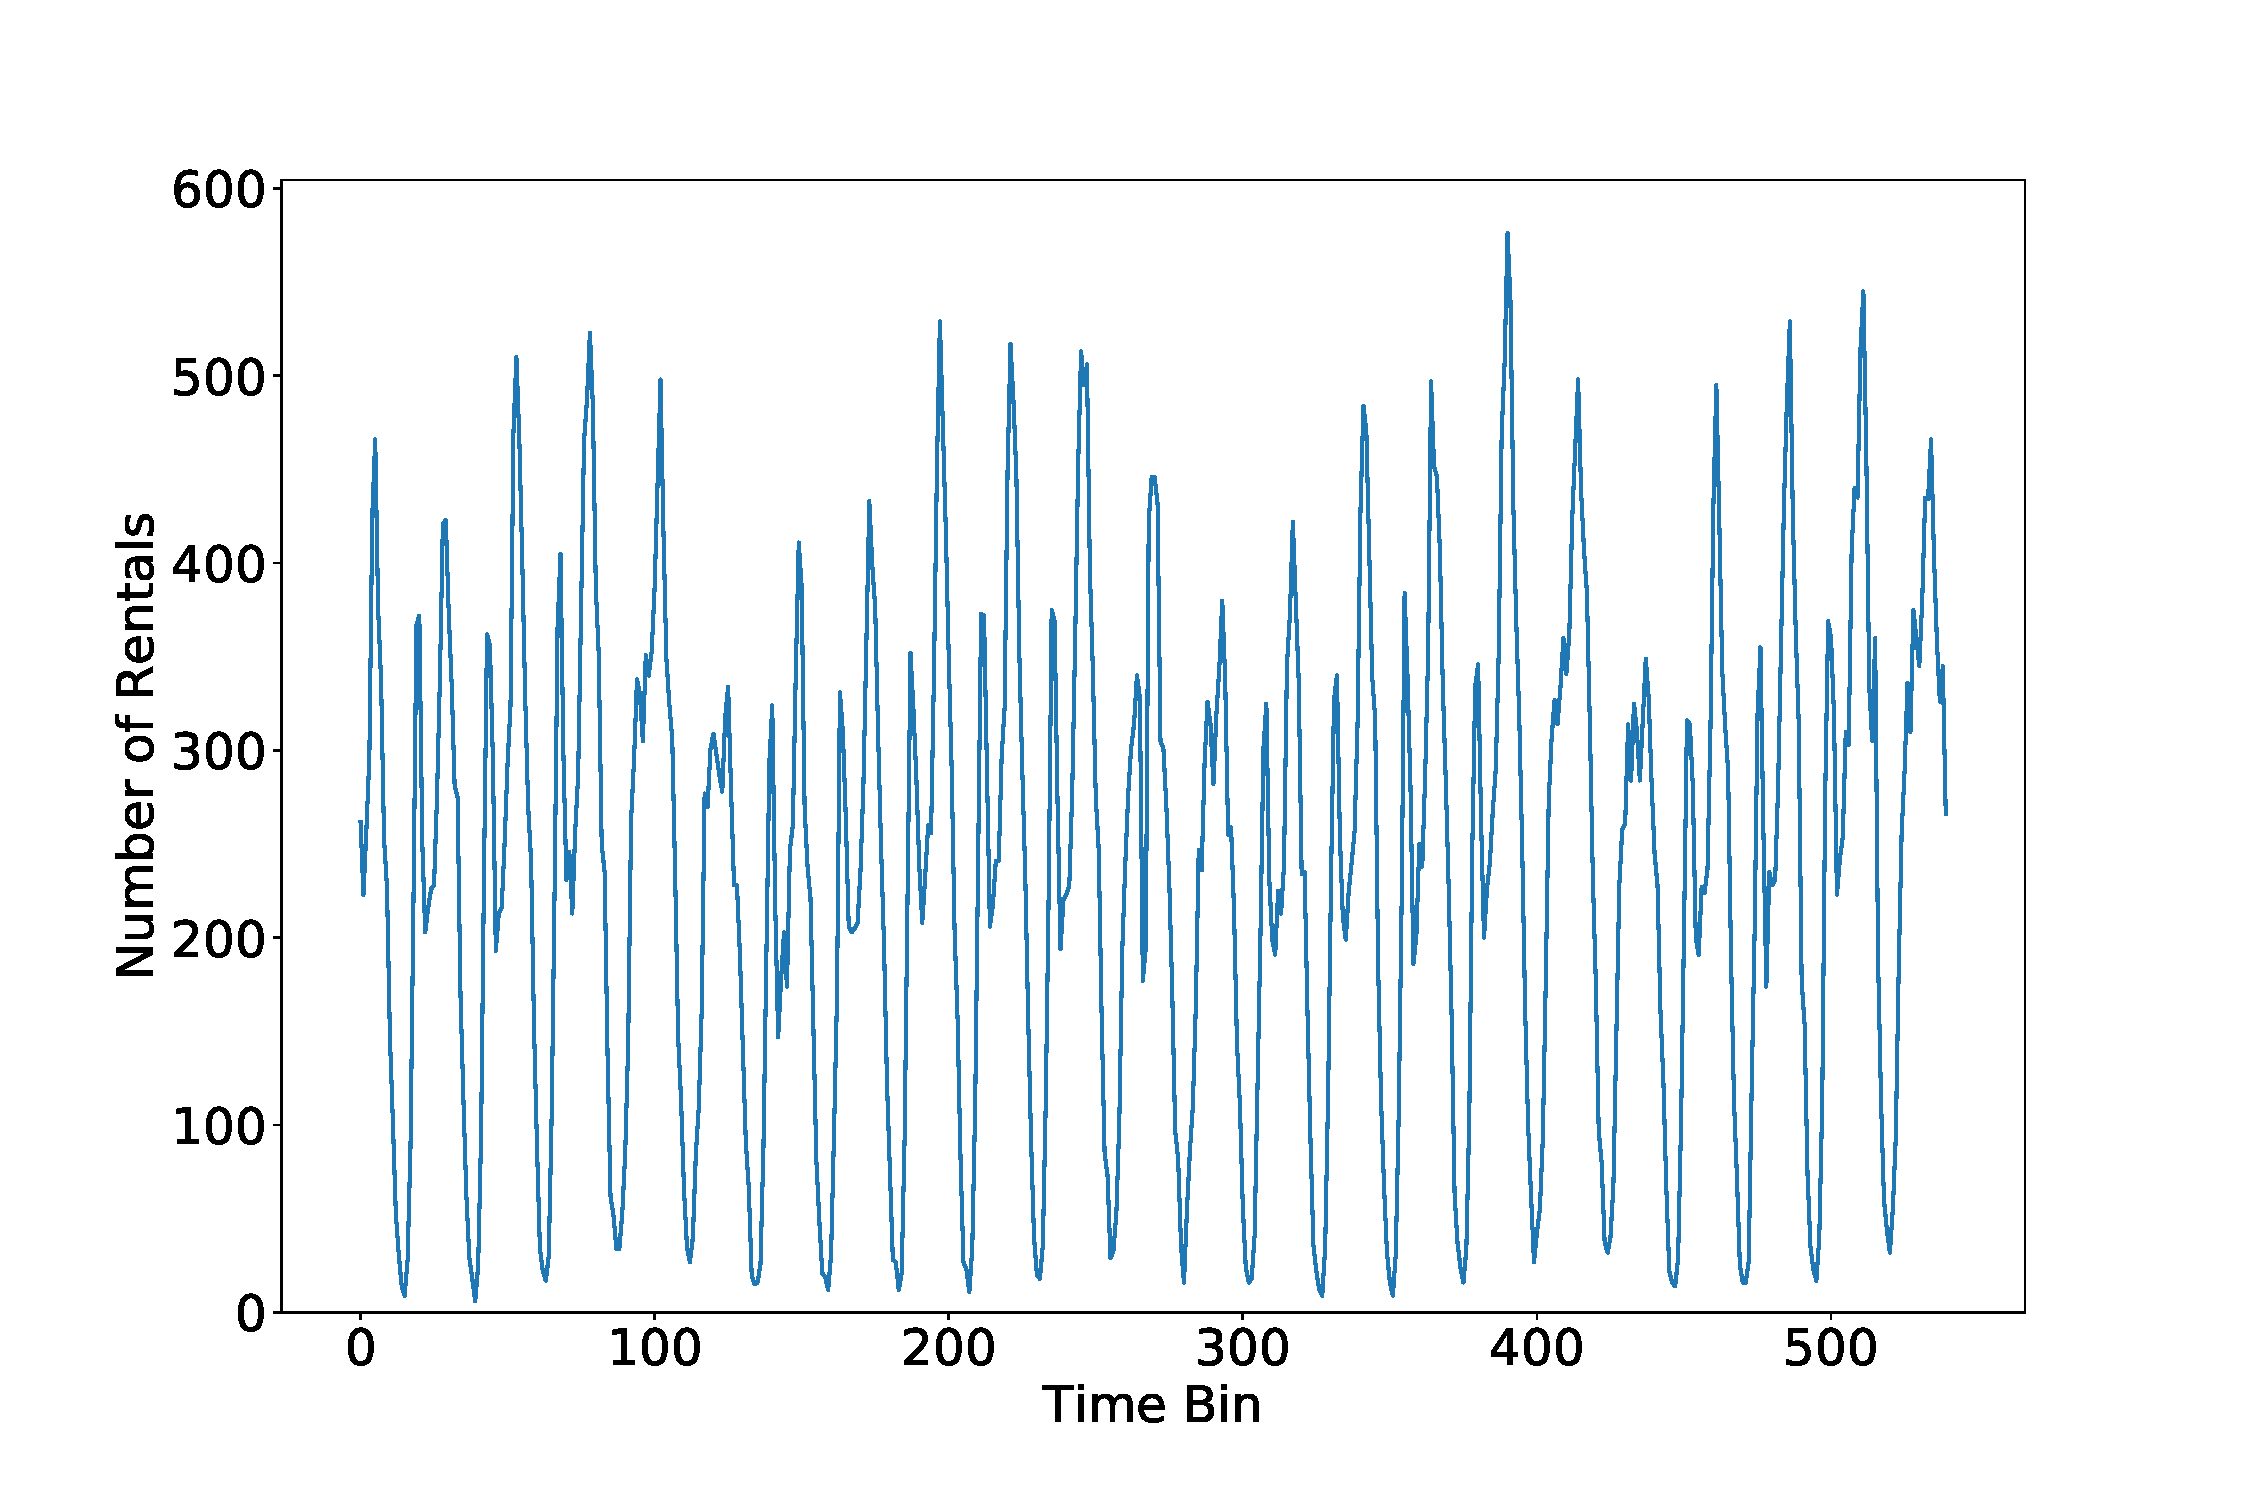
\includegraphics[width=0.65\columnwidth]{figures/temporal_characterization/BookingsHourAnalysisPeriod.pdf}
             \caption{Time series of starting rentals in September 2017 aggregated per hour. The difference in the total number of time bins and the actual number of hours in the month are due to missing data (crawler failures).}
            \label{fig:time_series}
    \end{center}
\end{figure}
%
\begin{figure}
    \begin{center}
        \begin{subfigure}{0.65\columnwidth}
            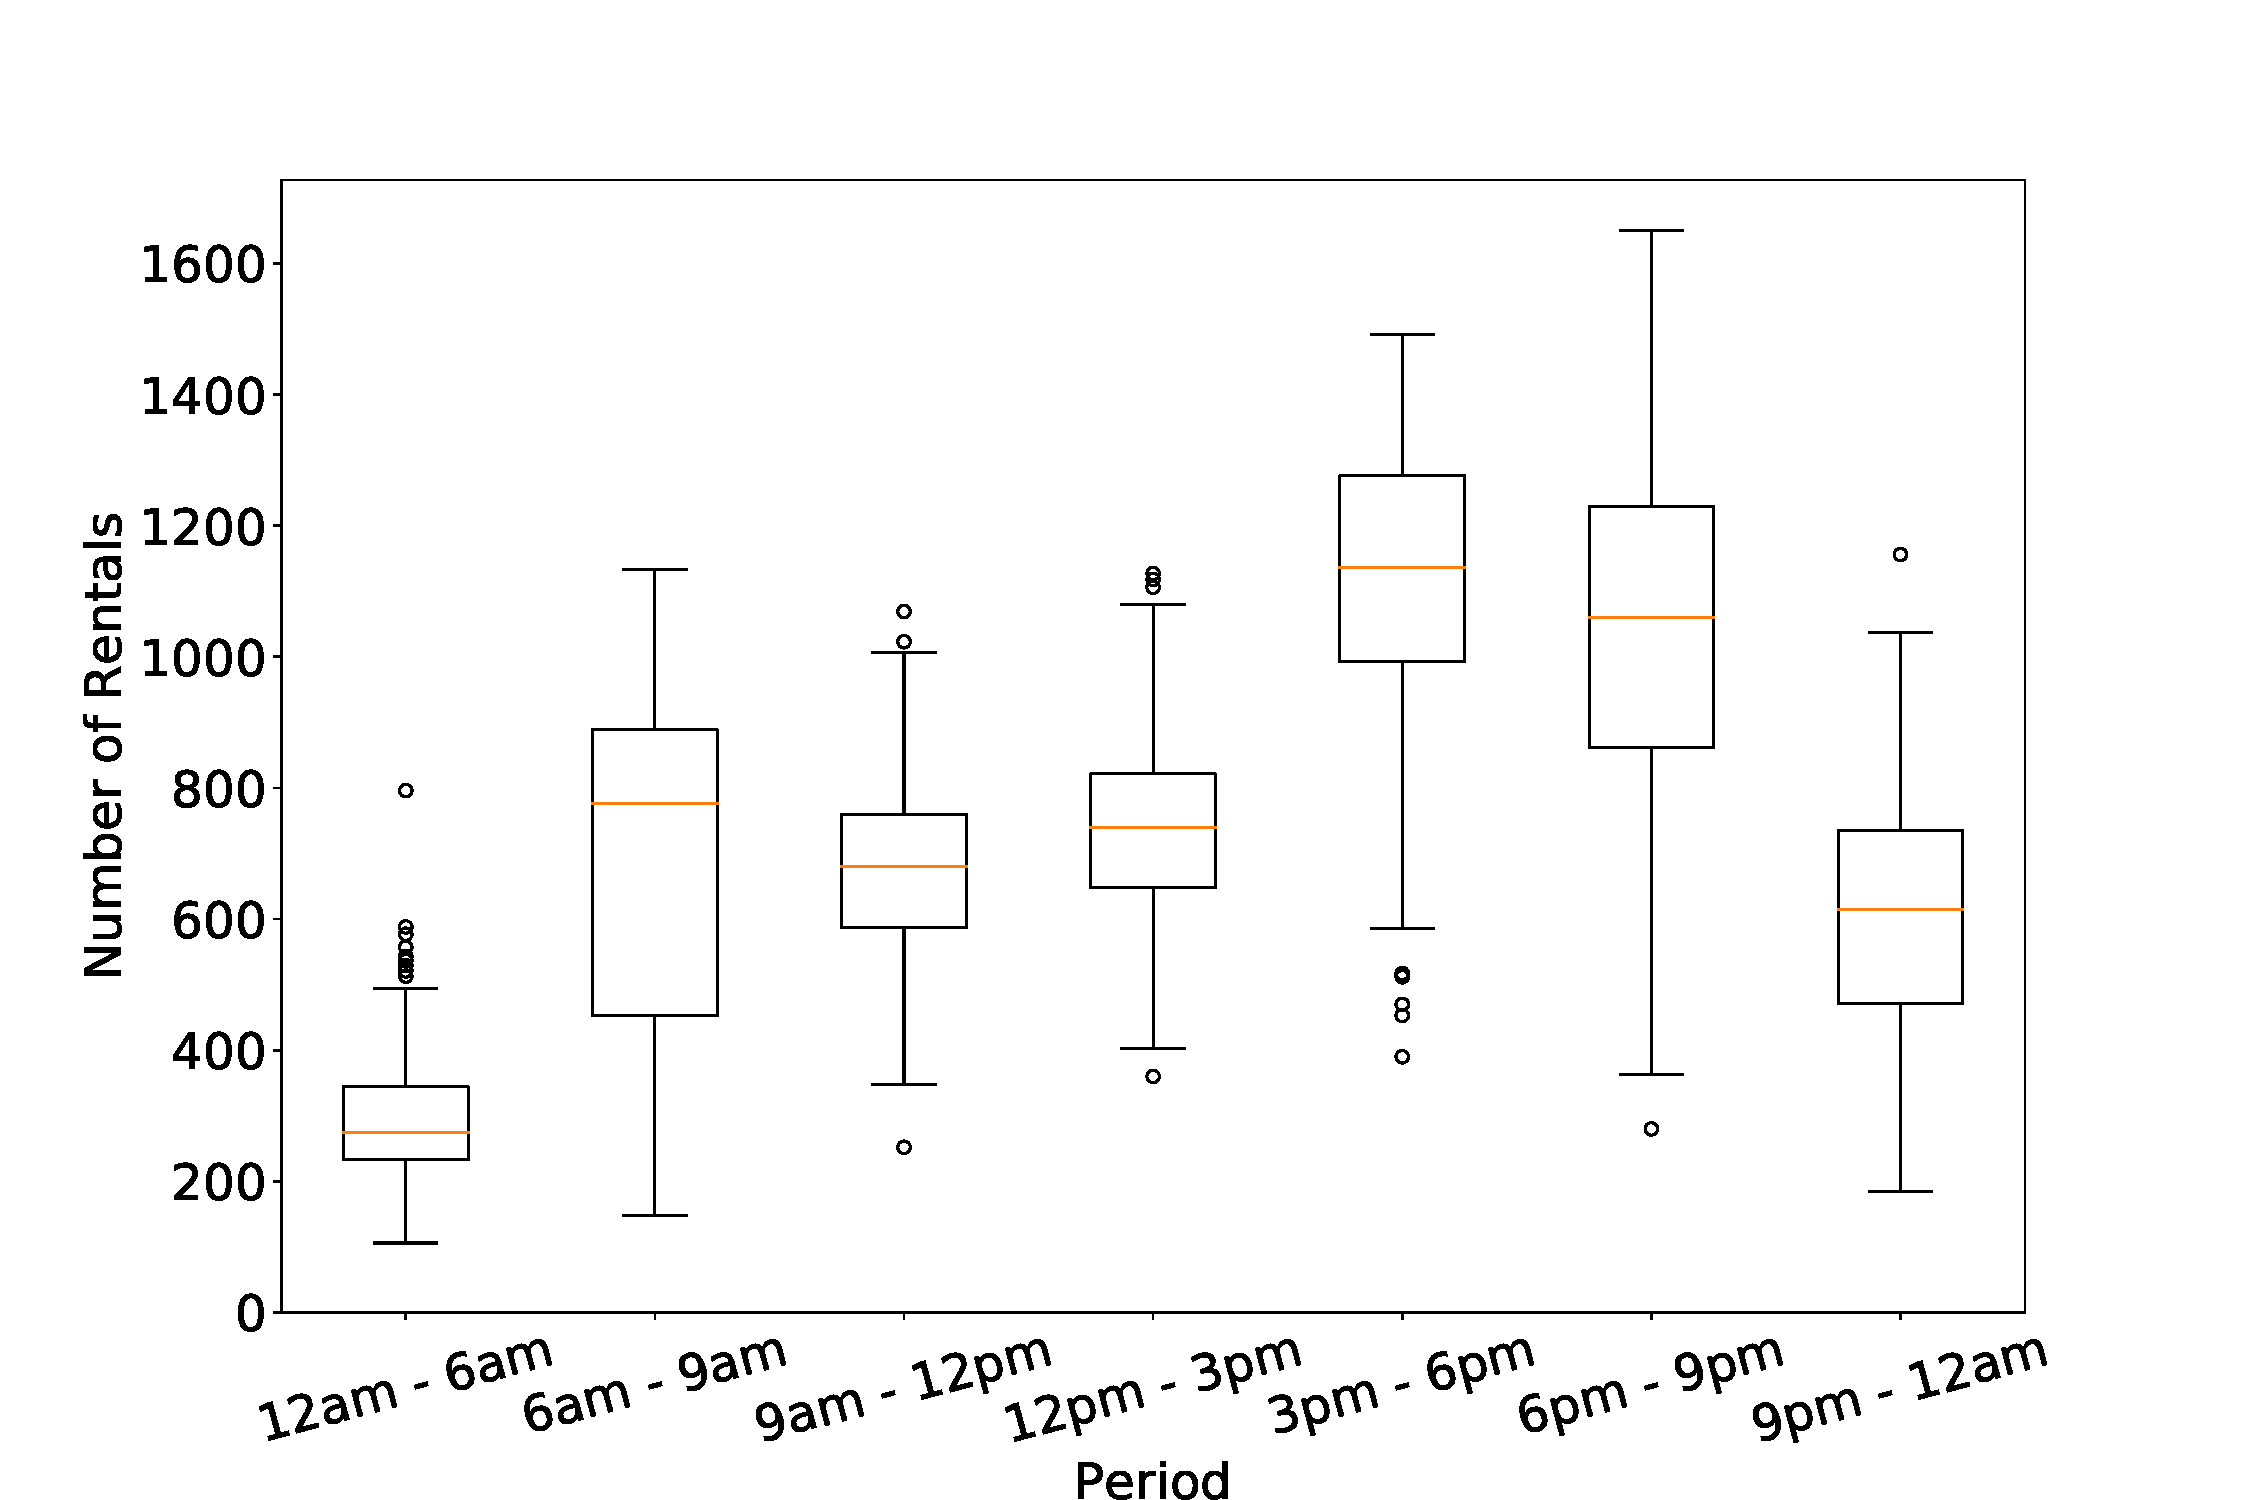
\includegraphics[width=\columnwidth]{figures/temporal_characterization/AverageBookingsPeriod.pdf}
             \caption{Boxplots of number of rentals starting in each time bin
             \vspace{0.5cm}}
             \label{fig:rentals-per-period}
        \end{subfigure}
        \begin{subfigure}{0.65\columnwidth}
            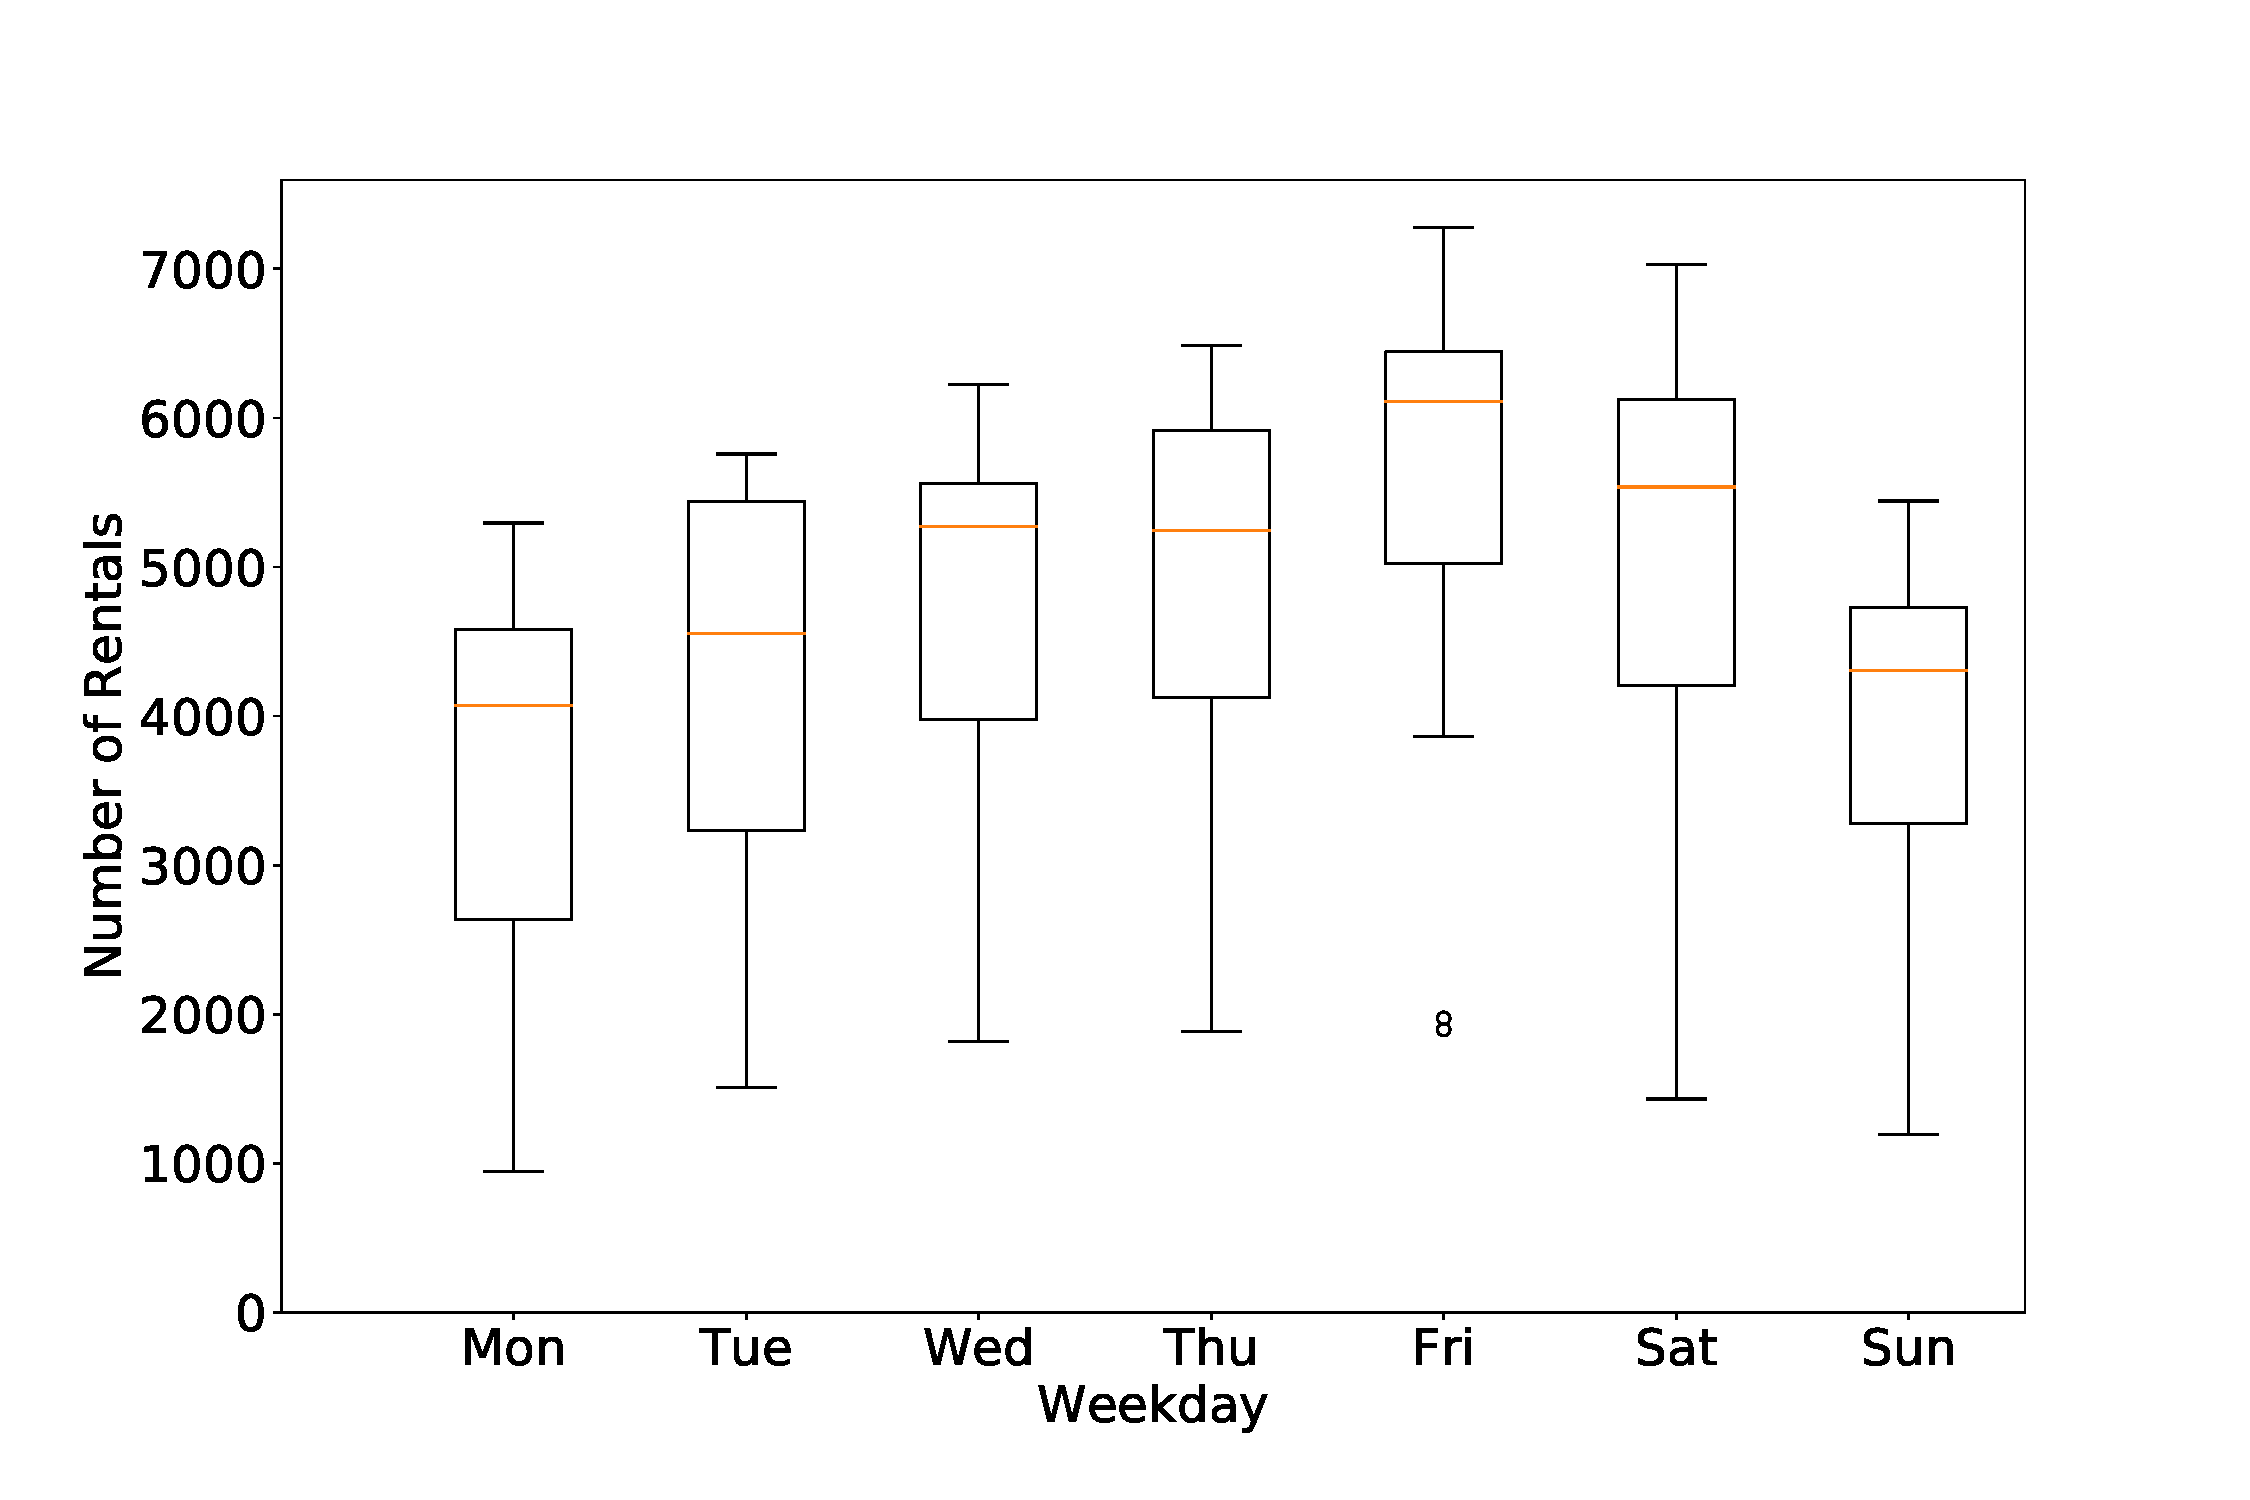
\includegraphics[width=\columnwidth]{figures/temporal_characterization/AverageBookingsWeekday.pdf}
             \caption{Boxplots of number of rentals starting in each day of the week}
             \label{fig:rentals-per-weekday}
        \end{subfigure}
        \caption{Temporal characterization of number of rentals. Boxplots highlighting the variability over the day for the same time bin of the day (top plots), and over different days (bottom plots).}
    \end{center}
\end{figure}


We start by showing the temporal evolution of rentals over time.  Figure~\ref{fig:time_series} shows the total number of starting rentals per hour in the whole city during part of September 2017. Even if we can spot some periodicity, there is a lot of variability that makes the prediction problem not straightforward. 
For our analyses, from now on we aggregate rentals both in time  and in space. Specifically, given a neighborhood we consider the fraction of rentals \textit{starting} and \textit{ending} there. We aggregate the time series of rentals into 7 time bins per each day, namely from midnight to 6am (night period), and then every 3 hours. 
This time granularity is typically used for system design and control~\citep{schmoller2015empirical}. The rationale is to provide the FFCS company that actionable information on the demand for cars, e.g., to schedule car maintenance or implement relocation policies. A one-hour period is often too short for the company to be able to respond to changes in demand.

To give more details about the variability of the data, Figure~\ref{fig:rentals-per-period} shows boxplots of the  numbers of rentals starting in each time bin. 
Each boxplot represents the quartiles of the distribution, with outliers shown as points.\footnote{We consider as outliers measures that are outside the mean $\pm$ 2.698 times the standard deviation range.} 
The series shows large variability, with peaks during early mornings (6am-9am) and afternoon (3pm-6pm and 6pm-9pm), and with low values during nighttime (12am-6am). 
Figure~\ref{fig:rentals-per-weekday} shows boxplots of the total number of rentals grouped per day of the week. The number of rentals peaks on Fridays, with significantly lower values registered on Sundays and Mondays. 
Again, we observe a quite sizeable variability over the days, as observed by in the sizes of the boxplots. 
Such variability in the number of rentals hints at the fact that prediction models have to be able to deal with sizeable temporal variations in the demand for cars.

\subsection{FFCS spatial characterization}

We now take a closer look into  how these numbers vary across 
different areas of the city. Rather than providing a complete characterization of the origin/destination matrix (which is outside the scope of this work), we here focus on particular examples to showcase the spatial variability in the demand for cars. We focus on  the morning and afternoon peak time bins (6am-9am and 6pm-9pm). 
For each neighborhood we compute the \textit{net flow} defined as the difference between the number of rentals starting from that neighborhood, and the number of rentals arriving at that neighborhood during the specified time period. We consider the cumulative net flow in September 2017. 
Figure~\ref{fig:flows} depicts the results with a heat map. Darker red neighborhoods mean that arrivals exceed departures, i.e., the neighborhood is attracting vehicles. Conversely, lighter colors imply that more vehicles are departing from that neighborhood than arriving in it. Numbers identify different neighborhoods.
The downtown business area (number 3) attracts a lot of rides in the morning period (Figure~\ref{fig:morning_flow}), while the opposite pattern is seen during the afternoon period (Figure~\ref{fig:afternoon_flow}). 
In general, we can assert that the FFCS demand is higher in the peak hours, and the cars flow towards downtown in the morning and towards residential areas in the afternoon. 
This is clearly visible in Figure~\ref{fig:net_flow} which reports the net flow for two neighborhoods for each hour of the day, namely the downtown neighborhood (number 3), and the Grandview-Woodland (number 21) neighborhood, a residential area close to downtown.

\begin{figure}
\begin{center}
        \begin{subfigure}{0.65\columnwidth}
            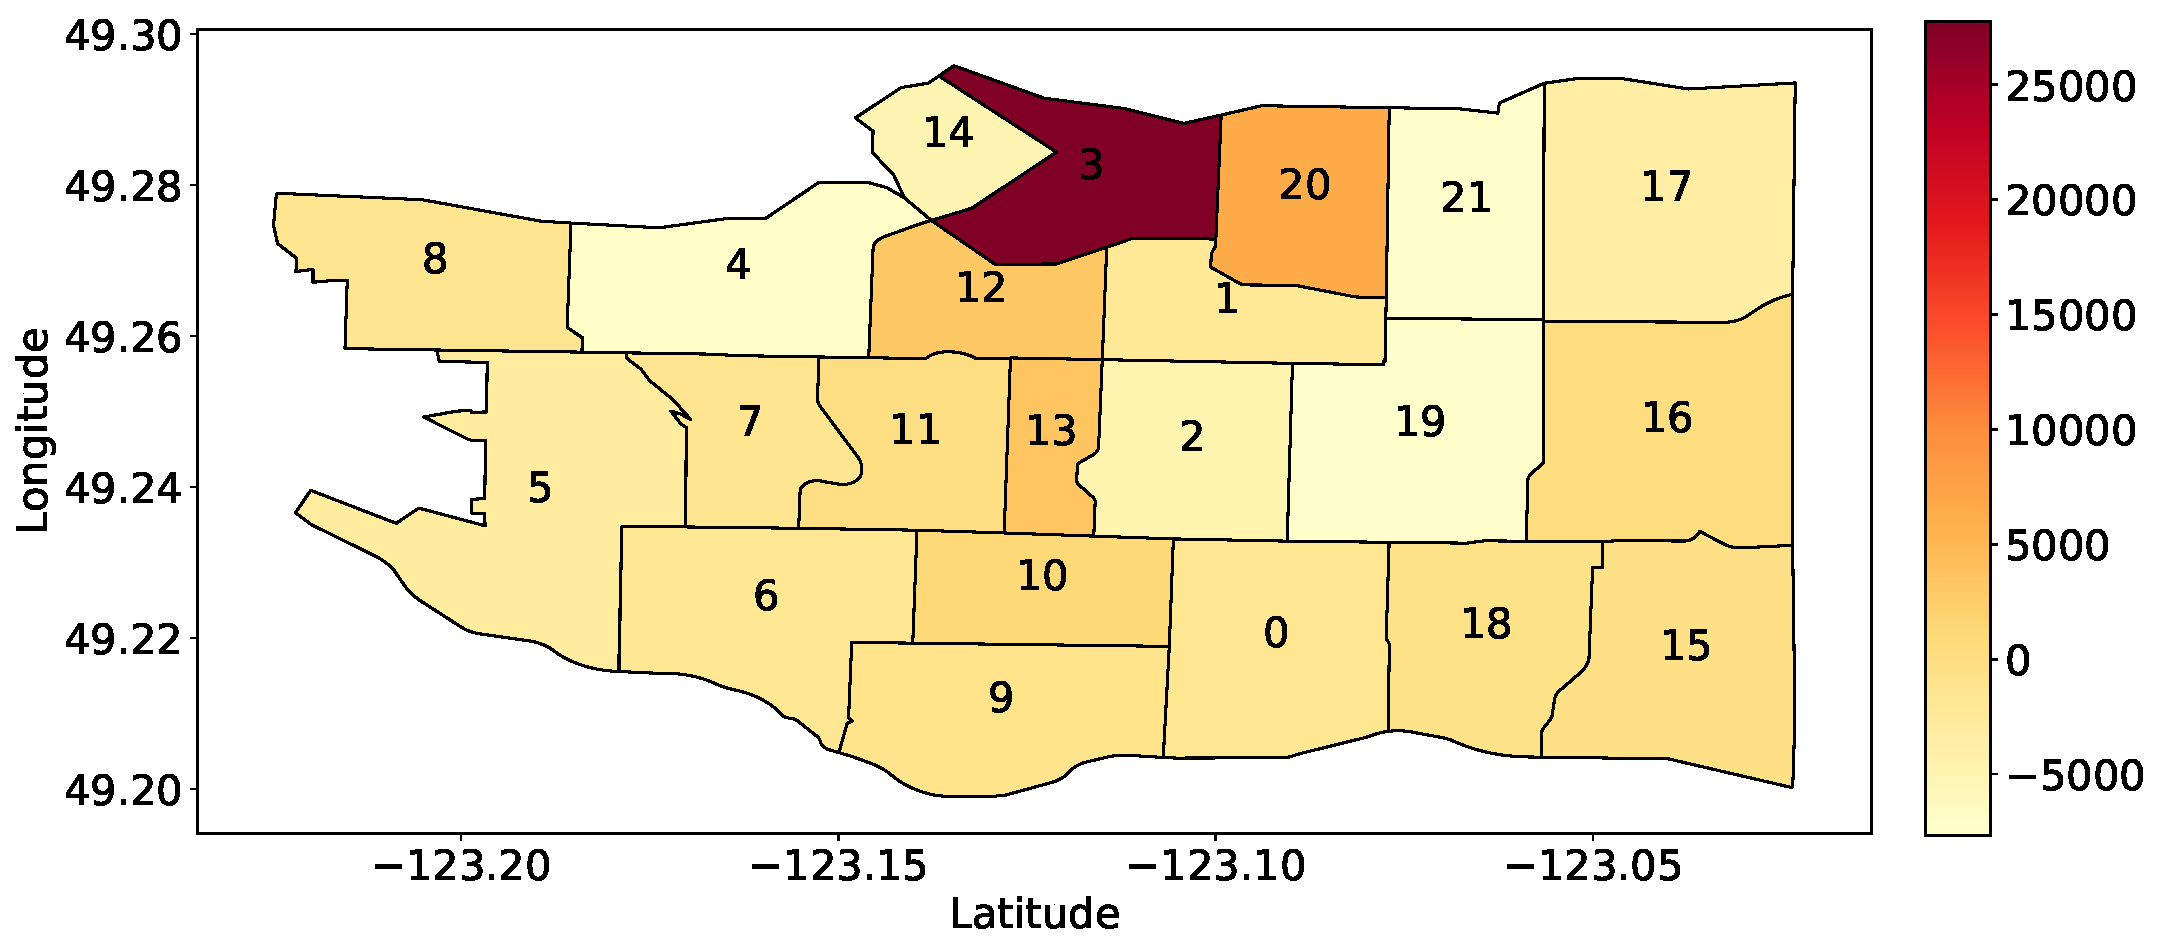
\includegraphics[width=\columnwidth]{figures/data_coll_char/morning_flow_n.pdf}
            \caption{6am - 9am rental net flow
            \vspace{0.5cm}}
            \label{fig:morning_flow}
        \end{subfigure}
         \begin{subfigure}{0.65\columnwidth}
             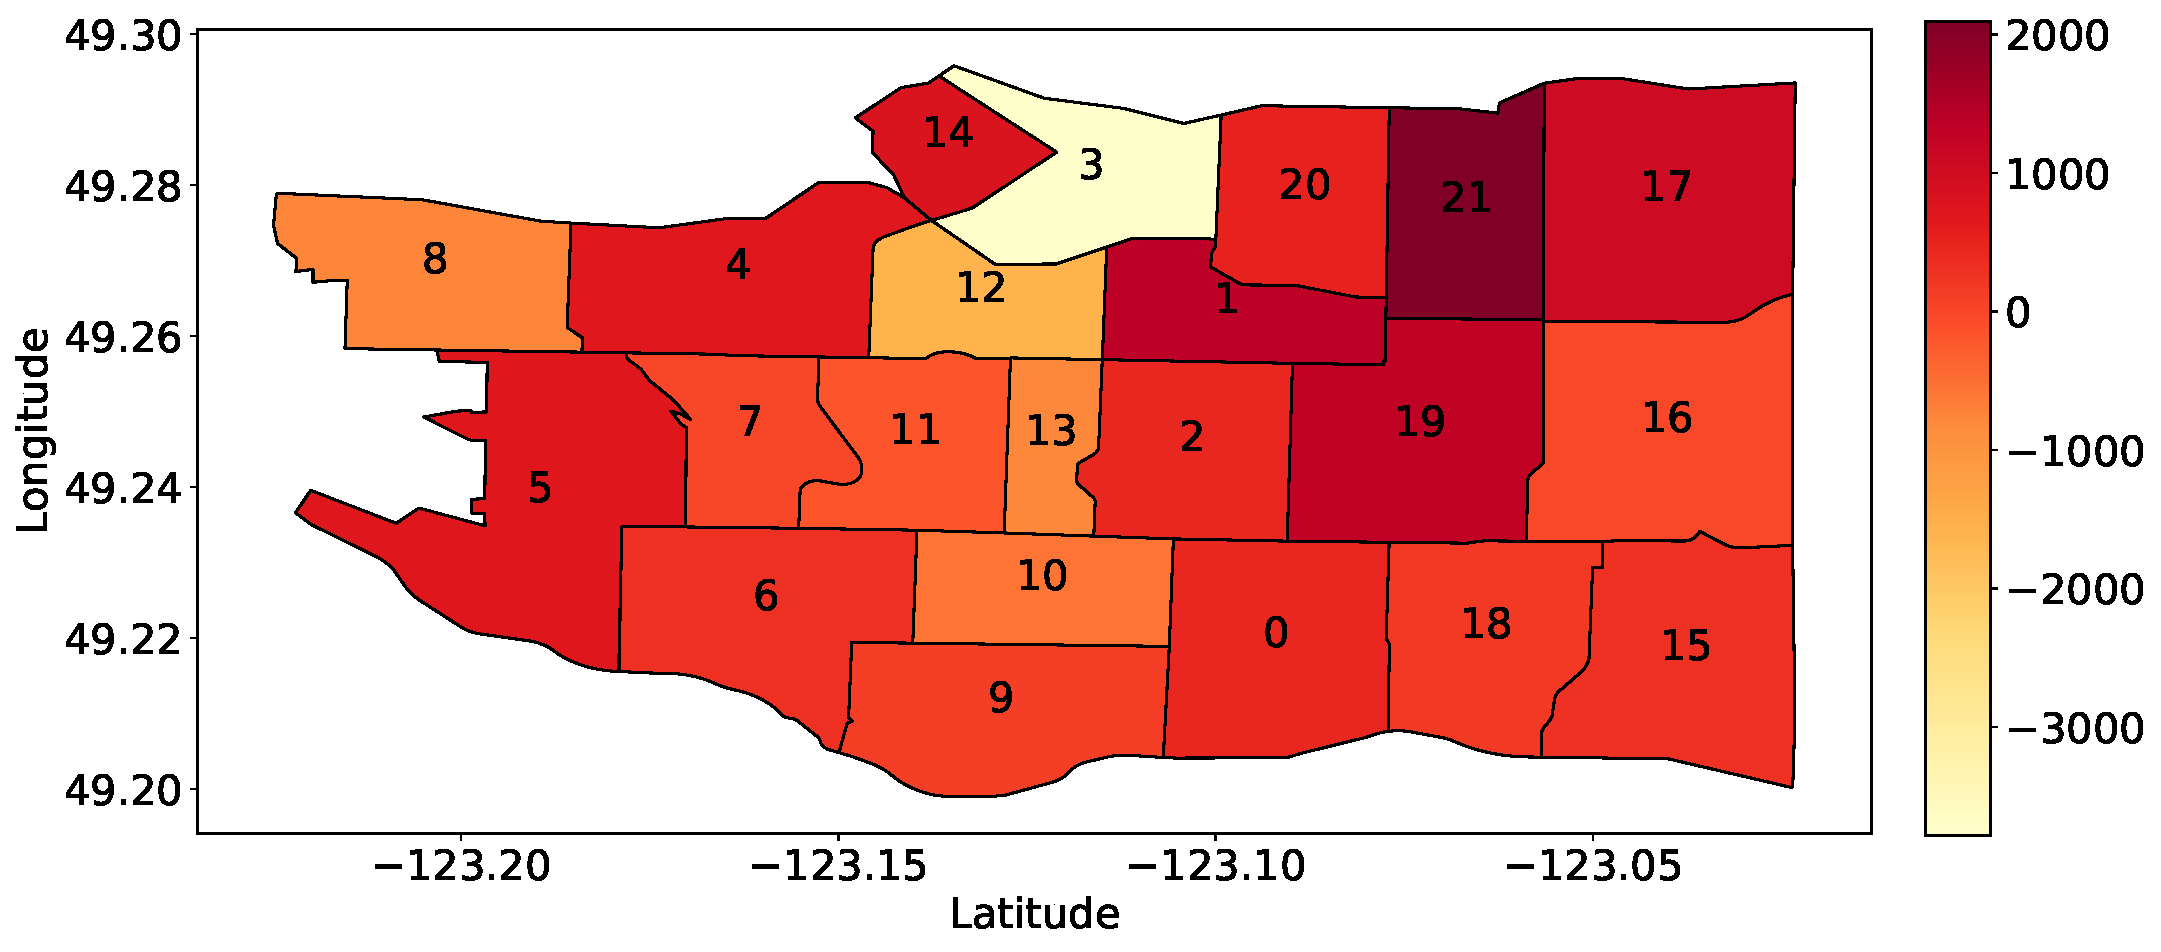
\includegraphics[width=\columnwidth]{figures/data_coll_char/afternoon_flow_n.pdf}
             \caption{6pm - 9pm rental net flow}
             \label{fig:afternoon_flow}
         \end{subfigure}
 	\caption{Heatmap of net flow for each neighborhood in Vancouver. The more the area is red, the higher are the arrivals with respect to the departures. Neighborhood numbering is shown (from 0 to 21) }
    \label{fig:flows}
    \end{center}
\end{figure}

\begin{figure}
    \centering 
    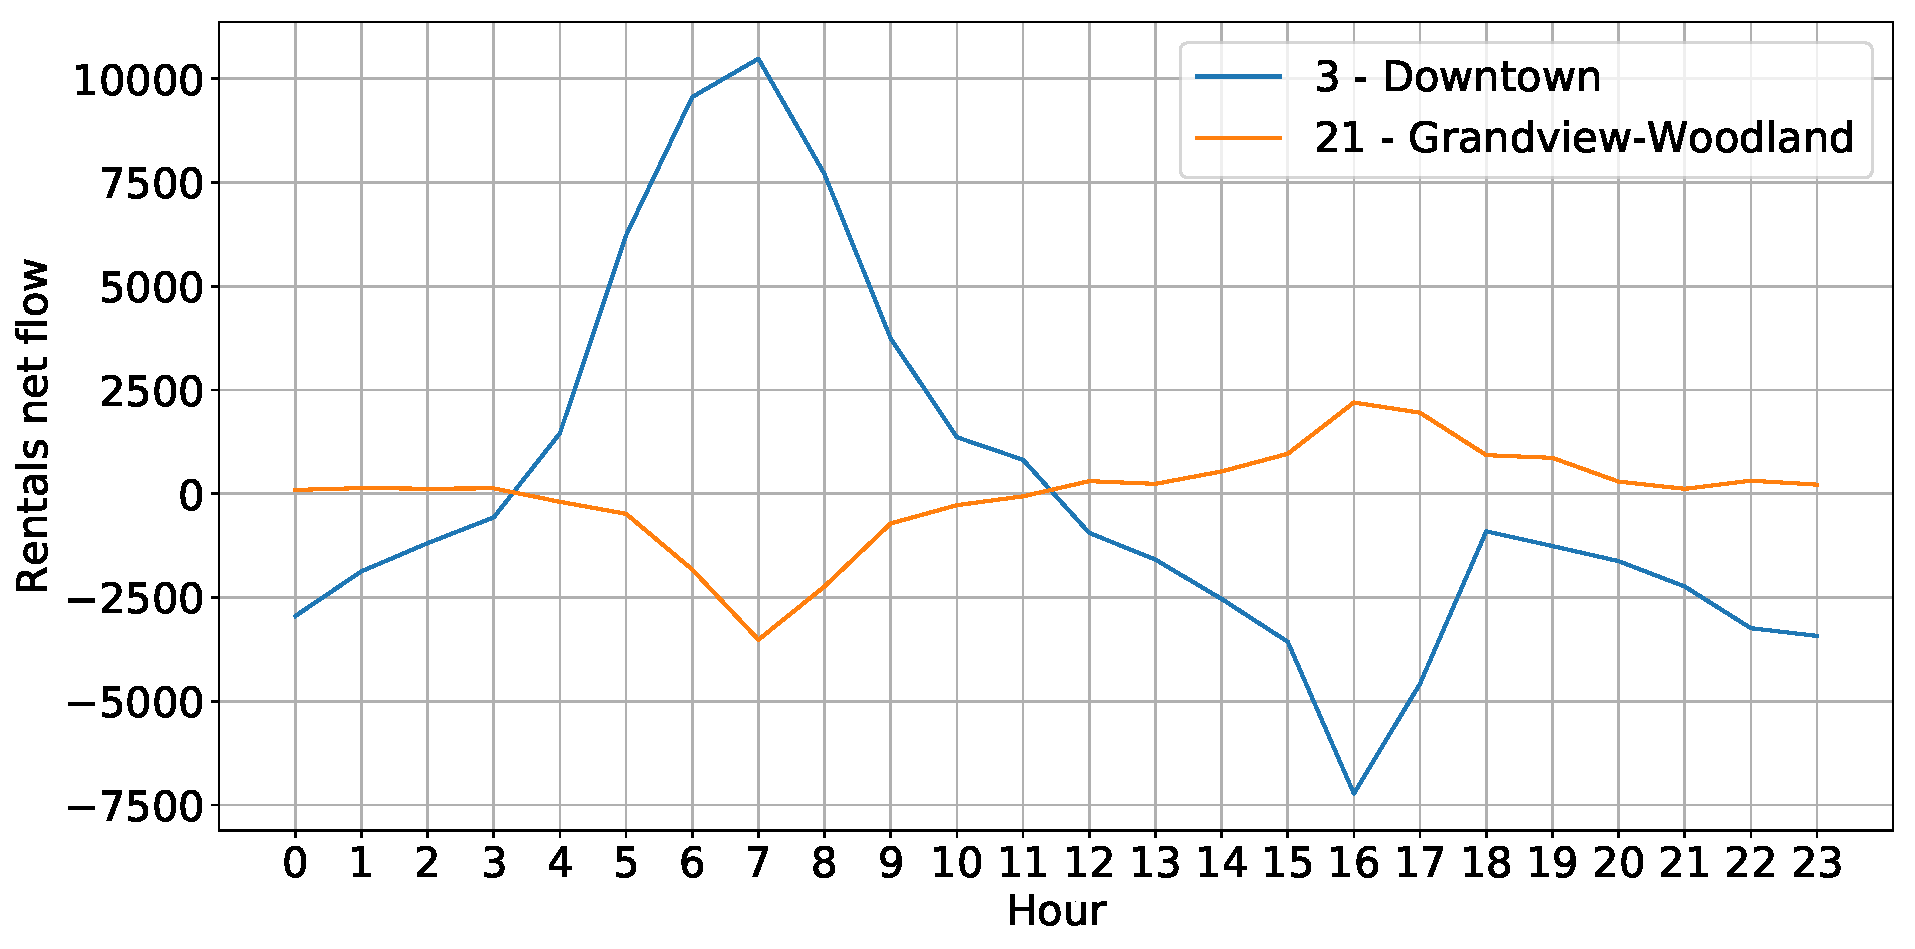
\includegraphics[width=0.65\columnwidth]{figures/data_coll_char/flows_per_zone.pdf}
    \caption{Total net flow in September 2017 for  Downtown (neighborhood 3) and Grandview-Woodland (neighborhood 21)  over different hours of the day}
    \label{fig:net_flow}
\end{figure}



\subsection{Socio-demographic and weather data characterisation}

We now provide some examples of the socio-demographic and open data. Figure~\ref{fig:weather-per-day} reports the weather condition during the month of September 2017. Being it a categorical variable, we assign to each weather condition a different value on the y-axis. As expected, the weather conditions change over time quite frequently. Moreover, no visible correlation is found when comparing the weather conditions with the number of rentals in Figure~\ref{fig:time_series}. 

Similarly, Figures~\ref{fig:richness-per-zone} and ~\ref{fig:calls-per-zone} show the number of high-income households and the number of emergency calls per day for each neighborhood, respectively. Also in this case, it is hard to see any clear correlation with the net flow per neighborhood reported in Figures~\ref{fig:flows}. 
The scenario is similar considering other socio-demographic features.

Despite the non-linear correlations between the socio-demographic data and rentals, it is possible that the combination of multiple features help the prediction of car rentals, as we will discuss in the next sections. 
This is exactly what the machine learning algorithms aim at, i.e., building a model from data, leveraging correlation from multiple variables that, considered together, carry enough information to predict system usage.
Thus, we let the machine learning model decide if and how to factor different features in the prediction model.

\begin{figure}
    \centering
    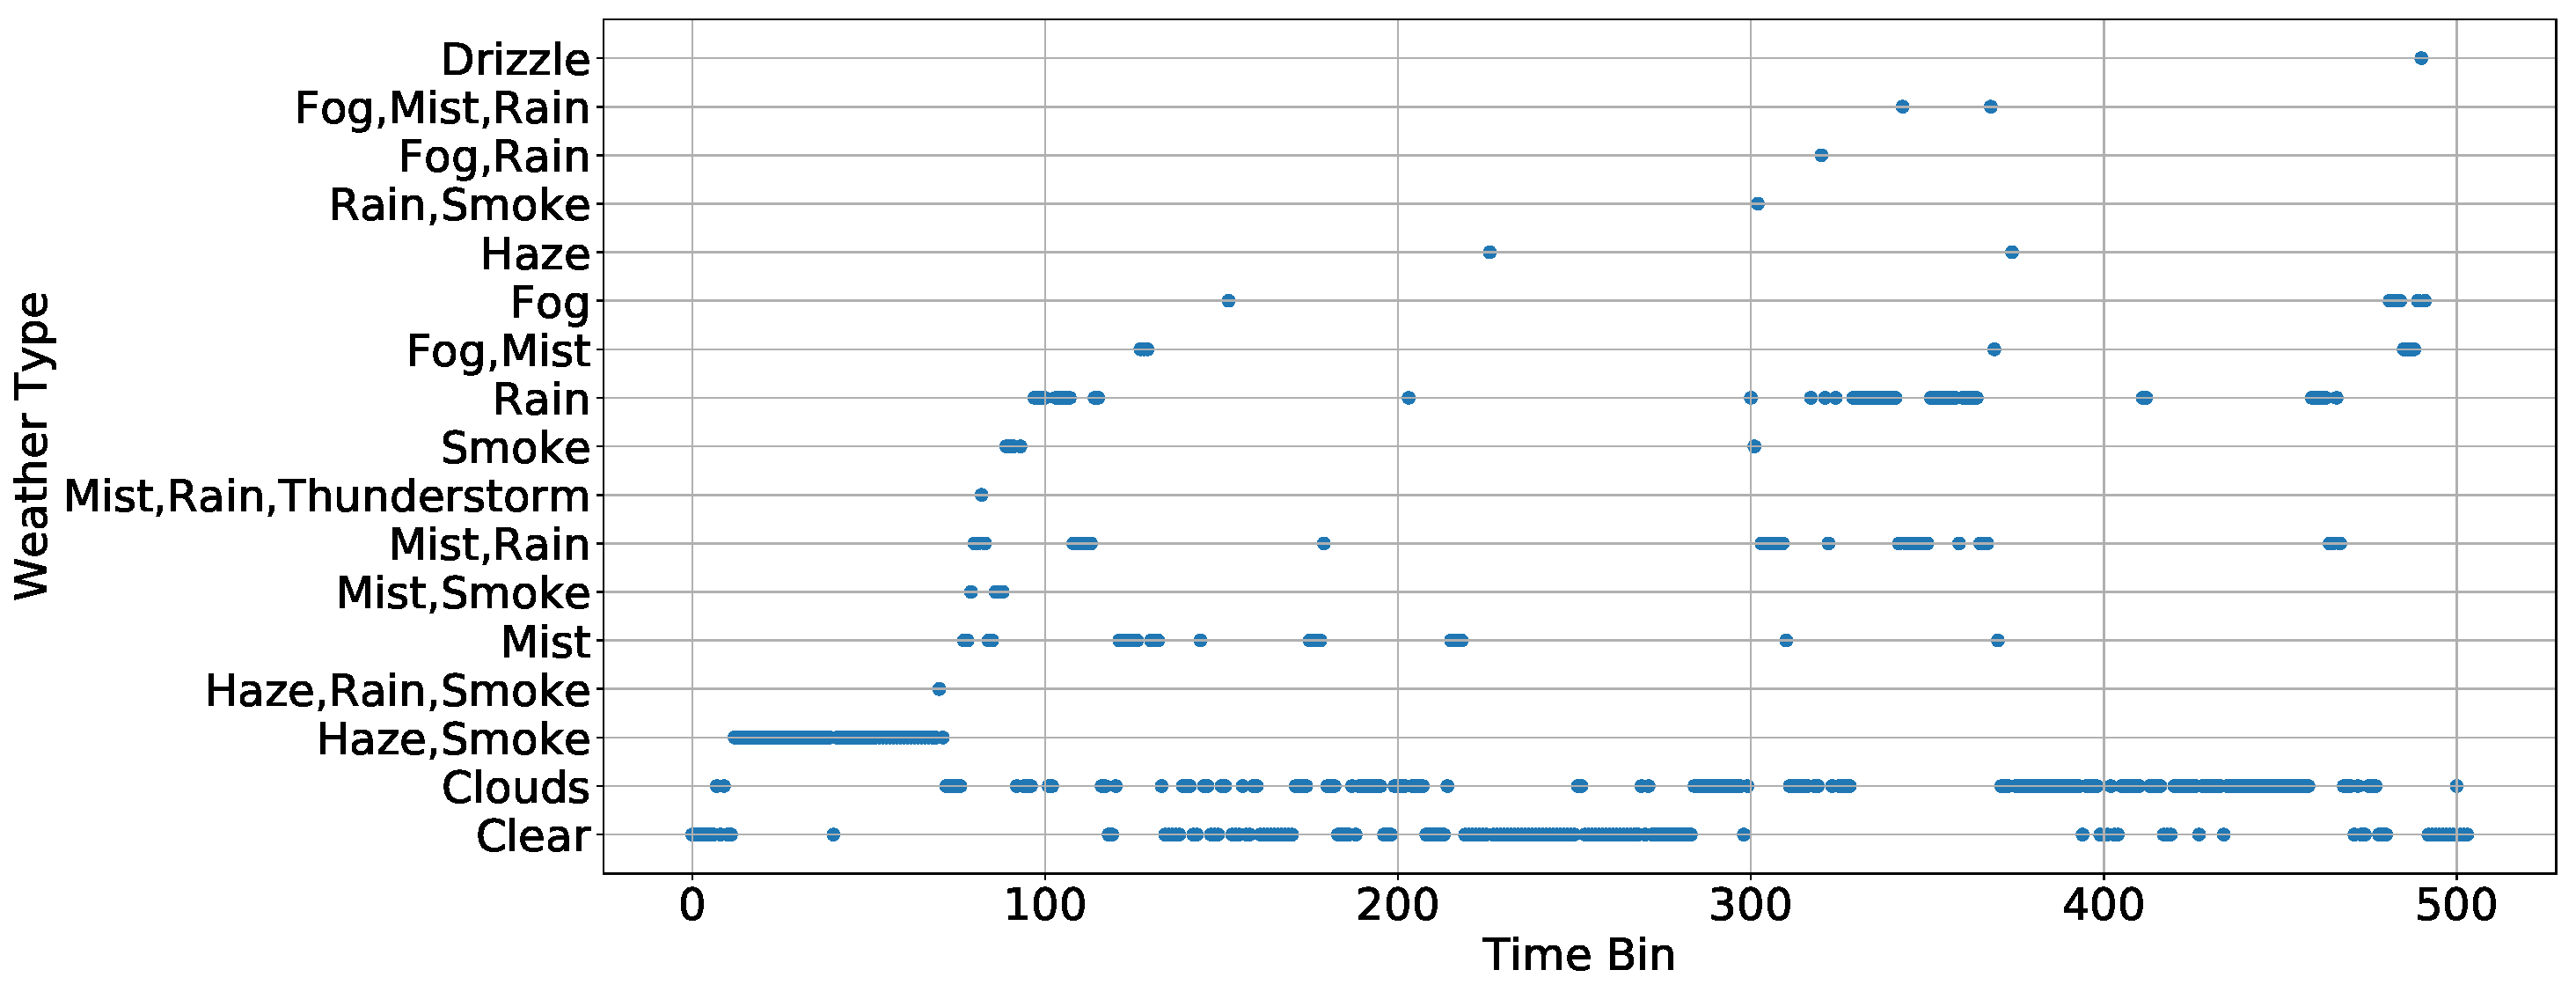
\includegraphics[width=0.8\columnwidth]{figures/temporal_characterization/WeatherPeriod2.pdf}
     \caption{Time series of weather conditions per hour during September 2017. Each point in the plot represents an occurred weather type.}
     \label{fig:weather-per-day}
\end{figure}


\begin{figure}
    \begin{center}
        \begin{subfigure}{0.65\columnwidth}
            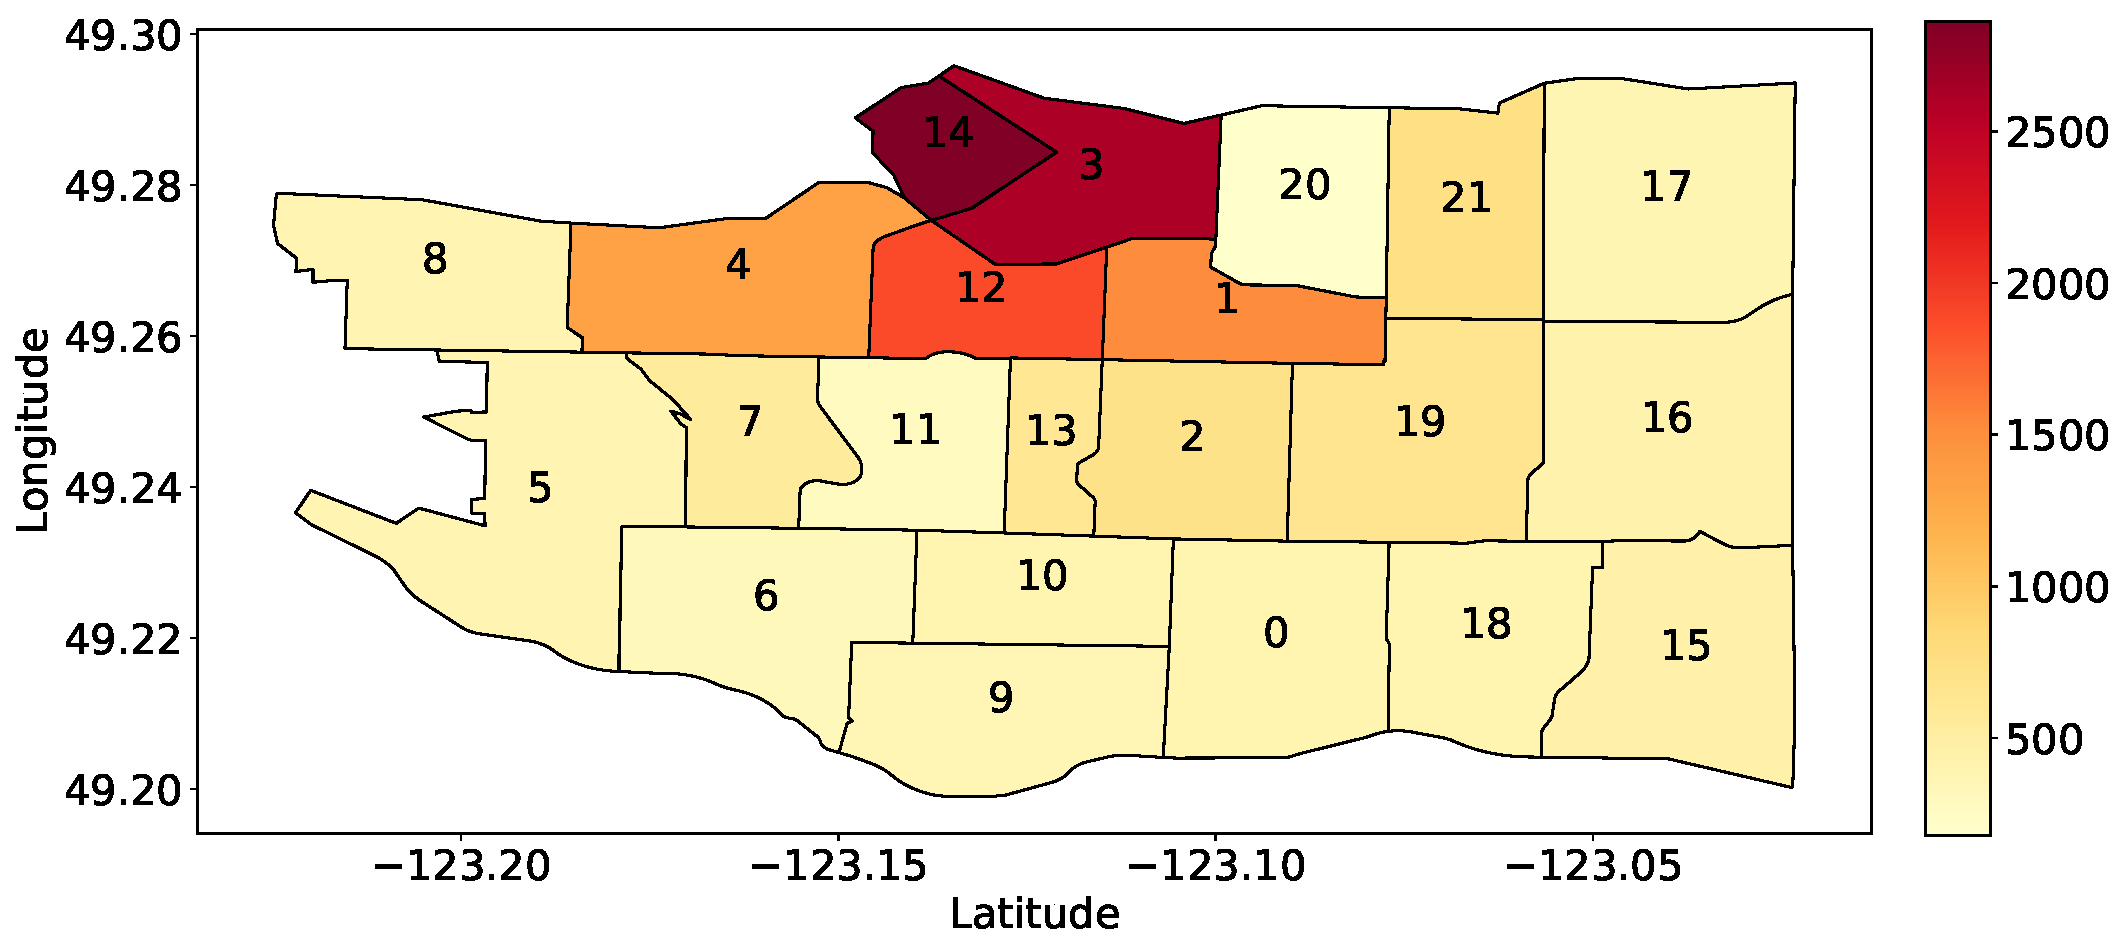
\includegraphics[width=\columnwidth]{figures/data_coll_char/Richness_80k+.pdf}
             \caption{Maximal income range density per neighborhood
             \vspace{0.5cm}}
            \label{fig:richness-per-zone}
        \end{subfigure}
        \begin{subfigure}{0.65\columnwidth}
            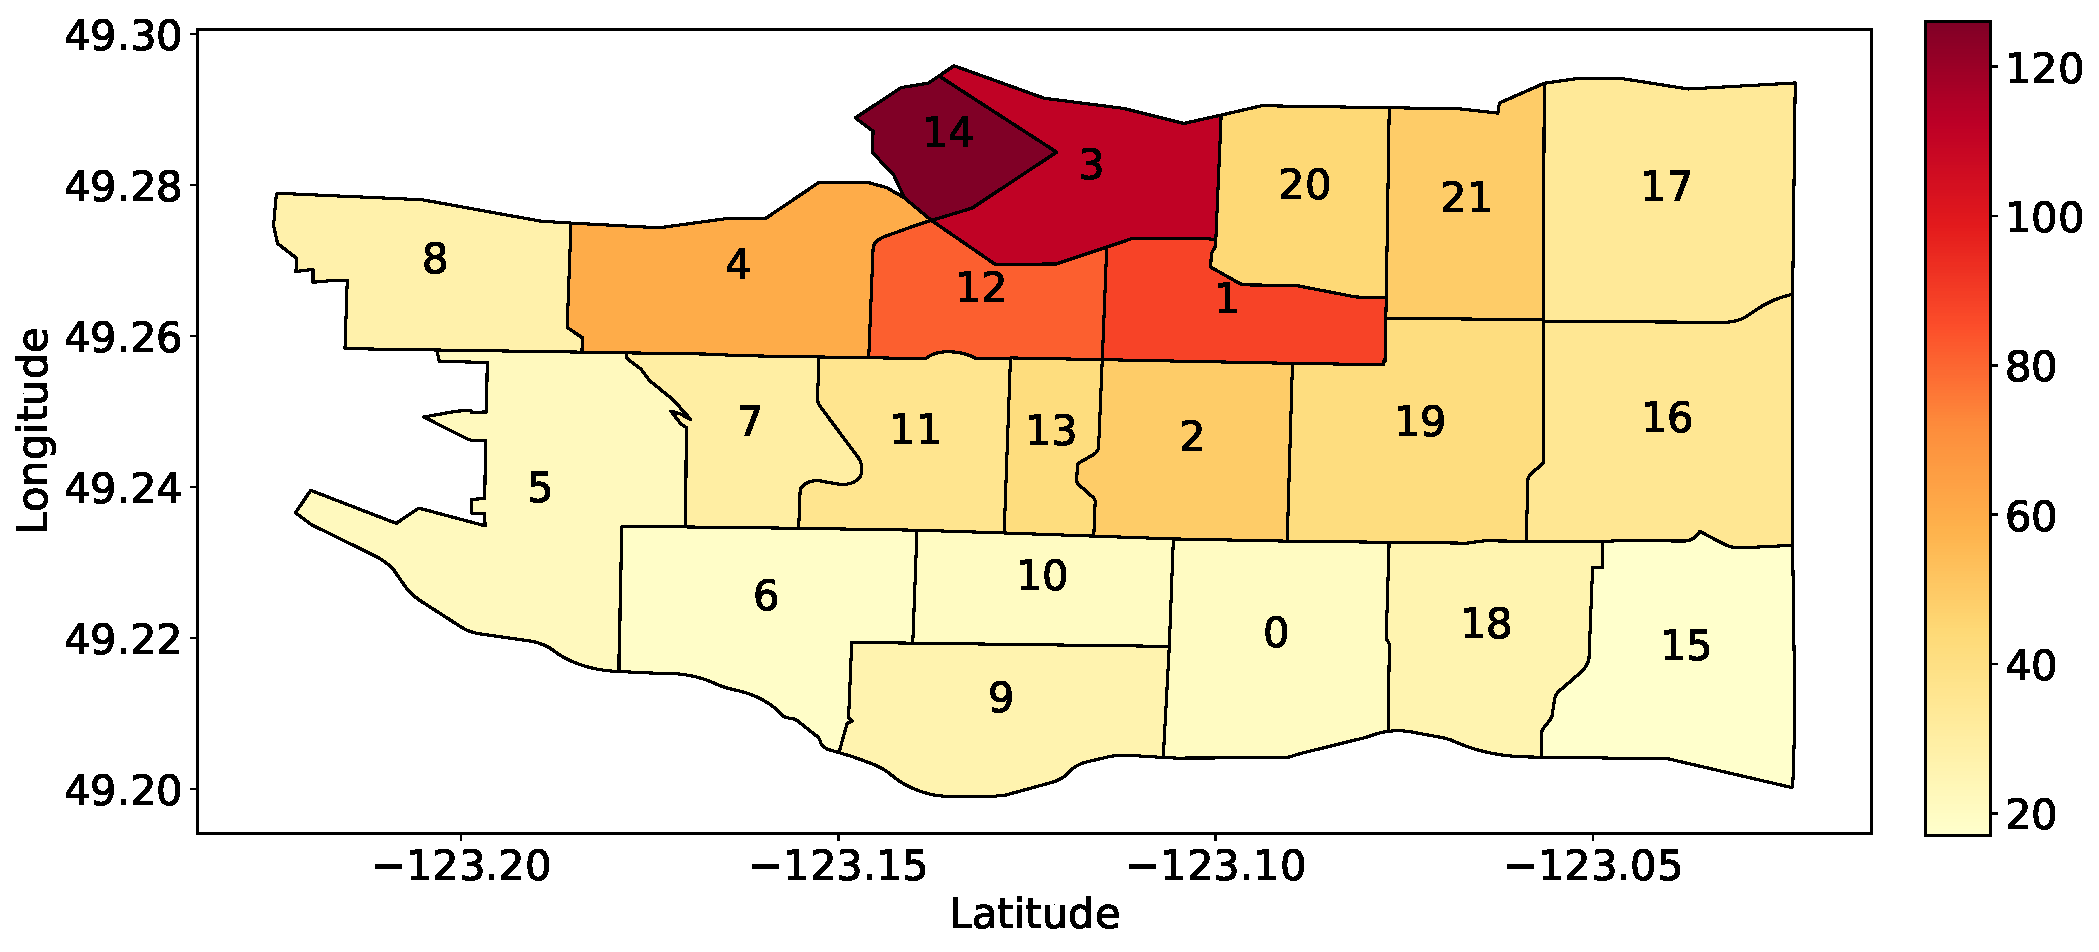
\includegraphics[width=\columnwidth]{figures/data_coll_char/emergencies.pdf}
             \caption{Emergency calls per day in each neighborhood}
            \label{fig:calls-per-zone}
        \end{subfigure}
        \caption{Heatmap of a sample of demographic (top) and socio-demographic (bottom) data at our disposals. These two samples look quite correlated.}
        \label{}
    \end{center}
\end{figure}

%\lv{Correlation between number of bookings and certain characteristics (young couples, no kids, etc). The motivation for this is that the carsharing company needs to move cars to certain regions of the city, and this information may help in finding which are those regions.}